\chapter{机器学习中的优化方法}

\begin{introduction}
  \item Gradient Descent
  \item Stochastic Gradient Descent
  \item Momentum
  \item Nesterov
  \item Adagrad
  \item RMSprop
  \item Adam
  \item AdamW
  \end{introduction}

我们可以把优化的问题简单的理解成一个“求最值”的问题。对于简单的情形,比如求$x^2+ax+b$的最小值,我们很容易能够得到这个问题的解析解$b-\frac{a^2}{4}$。但对于大多数机器学习问题,由于模型结构复杂,参数众多,甚至带有复杂的约束条件,我们很难得到解析解。此时,我们会采用一阶或者二阶优化方法,逐步逼近最优解。尤其在深度学习时代,采用更加便捷的一阶优化方法成为主流。当然这也是由于深度模型过于大和复杂导致的迫不得已的选择。

\section{梯度下降方法 (Gradient Descent Method)}

梯度下降算法是一个一阶优化算法,我们针对损失函数$J(\bm\theta)$,会首先将参数初始化为$\bm\theta_{0}$,之后采用迭代的方法不断更新参数$\bm\theta$。
\begin{equation}
  \label{grad_descent}
  \bm\theta_{t+1} \leftarrow \bm\theta_{t} - \nabla_{\bm\theta}J(\bm\theta)
\end{equation}

\begin{exercise}\label{exer:sgd}
  请证明优化目标函数$J(\bm{\theta})$在当前参数$\bm{\theta}$下的最优参数更新方向为梯度反方向$-\nabla_{\bm\theta}J(\bm\theta)$。  
\end{exercise}
 
\begin{proof}
  即 $D(x)$ 在 $[0,1]$ 上是 Lebesgue 可积的并且积分值为零。但 $D(x)$ 在 $[0,1]$ 上不是 Riemann 可积的。
\end{proof}

\section{随机梯度下降方法 (Stochastic Gradient Descent Method)}
梯度下降方法在每一步迭代过程中,会计算优化目标函数关于所有样本${\bm{x}_{i}}$的梯度,这会随着数据集中样本数量$n$的增长而线性增加,即计算复杂度为$\mathcal{O}(n)$。这导致的问题是,参数的一次迭代更新会非常耗时,且消耗大量计算资源。随机梯度下降方法则在参数迭代过程中只针对当前一个样本计算梯度$\nabla f(\bm{x}_i)$,并以此更新模型参数。在样本是随机同分布的情况下,随机梯度的期望显然等同于在全部数据集上的。

\section{Momentum}
在梯度下降的基础上,引入“速度”的概念。在梯度下降时,不以当前的梯度${\bm{x}_{i}}$进行参数更新,而是以速度${\bm{m}}$进行更新:

\begin{align}
  \label{momentum}
  \bm{m} &\leftarrow \beta\bm{m} - \eta\nabla_{\bm{\theta}}{J(\bm{\theta})},\\
  \bm{\theta} &\leftarrow \bm{\theta} + \bm{m}. \notag
\end{align}

书中经常举的例子是,对于一个狭长的半椭球体(elongated half-ellipsoid)损失函数,例如$f(\bm{x})=0.1x_{1}^{2}+2x_2^2$,采用Momentum优化方法会使得在较小梯度方向$\frac{\partial f(\bm{x})}{\partial x_1}$不断加速。而在较大梯度方向$\frac{\partial f(\bm{x})}{\partial x_2}$上,通过梯度间的不断抵消,避免了在$x_2$上的不必要的大梯度,且减弱了梯度震荡的影响。
Momentum方法引入了一个新的参数$\beta$,通常令$\beta = 0.9$是一个不错的选择。

\section{Nesterov}

Nesterov优化是基于Momentum优化的改进:对于计算梯度的选点,由当前参数$\bm{\theta}$更改为$\bm{\theta}+\beta\bm{m}$。这是因为使用Momentum方法更新参数时,当前速度$\beta\bm{m}$也会对参数进行更新,进行上述梯度修正,往往会得到一个更好的参数更新方向。

\begin{align}
  \label{nesterov}
  \bm{m} &\leftarrow \beta\bm{m} - \eta\nabla_{\bm{\theta}}{J(\bm{\theta}+\beta\bm{m})},\\
  \bm{\theta} &\leftarrow \bm{\theta} + \bm{m}. \notag
\end{align}

\begin{figure}[htbp]
  \centering
  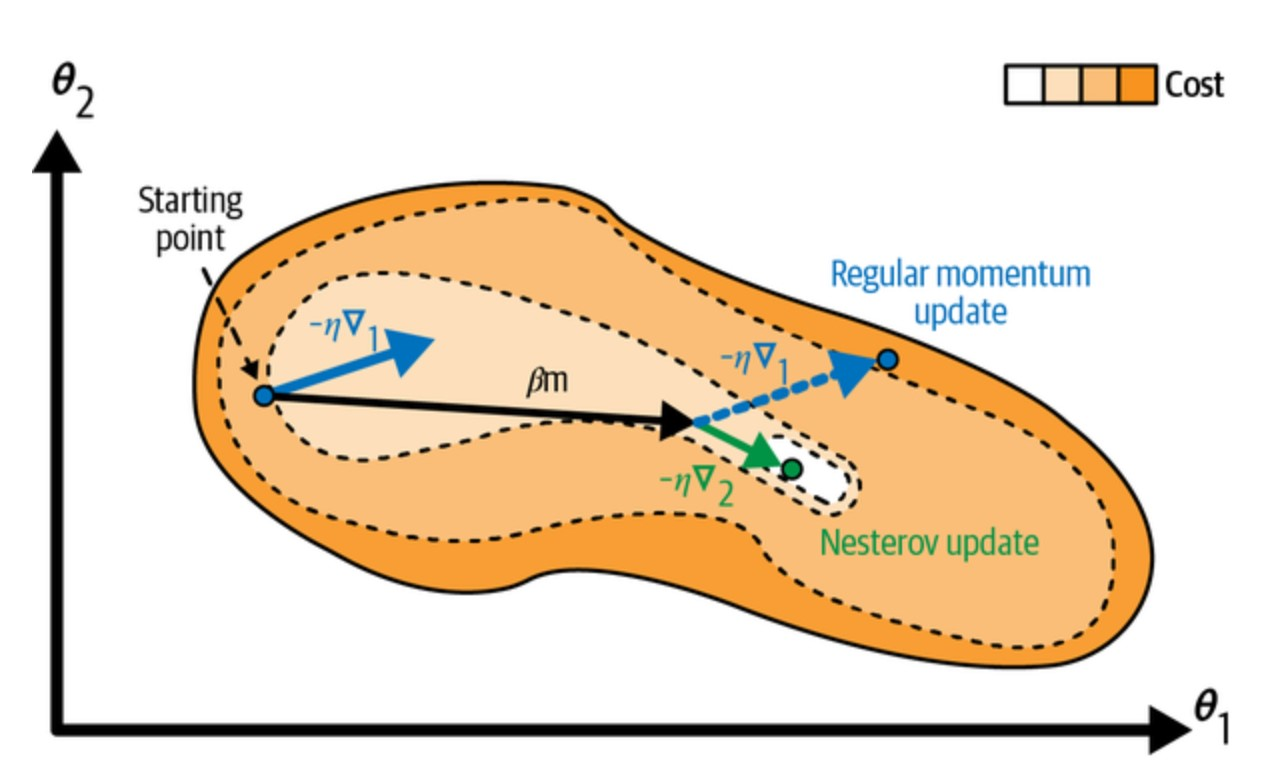
\includegraphics[width=0.6\textwidth]{nesterov.jpg}
  \caption{Nesterov优化方法相较Momentum方法具有更好的参数更新方向 \label{fig:nesterov}}
\end{figure}

图 \ref{fig:nesterov} 形象化说明了Nesterov比Momentum在计算参数更新方向上的优势\cite{geron2022hands} \footnote{图片来源于\cite{geron2022hands}}。


\section{Adagrad}

Adagrad 是在梯度下降的基础上的改进:对于参数在不同的维度上施加不同的decay rate。对于某些更加陡峭的维度,decay rate会相对更大,对于较为平缓的维度,decay rate会相对更小。

\begin{align}
  \label{adagrad}
  \bm{s} &\leftarrow \bm{s} + \nabla_{\bm{\theta}}{J(\bm{\theta})} \odot \nabla_{\bm{\theta}}{J(\bm{\theta})},\\
  \bm{\theta} &\leftarrow \bm{\theta} - \eta\nabla_{\bm{\theta}}{J(\bm{\theta})} \oslash \sqrt{\bm{s} + \epsilon} . \notag
\end{align}

由\ref{adagrad}可以看出,Adagrad中用于decay梯度的$\bm{s}$会随着迭代不断累积,这导致一个问题就是AdaGrad往往会early stop到一个不是很好的解。在实际应用中,尤其是深度学习场景,不推荐使用该优化方法。

\section{RMSprop}

RMSprop是基于AdaGrad的改进。在AdaGrad中,计算用于平衡不同维度间下降速率的decay weight的$\bm{s}$是不断累积的,因而会blew up进而使得模型训练过早地停止。RMSprop在$\bm{s}$的更新中引入了exponential decay,从而避免产生过大的decay weight,进而缓解了stop too early的问题。

\begin{align}
  \label{rmsprop}
  \bm{s} &\leftarrow \rho\bm{s} + (1-\rho) \nabla_{\bm{\theta}}{J(\bm{\theta})} \odot \nabla_{\bm{\theta}}{J(\bm{\theta})},\\
  \bm{\theta} &\leftarrow \bm{\theta} - \eta\nabla_{\bm{\theta}}{J(\bm{\theta})} \oslash \sqrt{\bm{s} + \epsilon} . \notag
\end{align}

RMSprop相较之前的优化方法,多了一个参数$\rho$。这个参数不需要过多调整,我们通常将其设置为0.9。

\section{Adam}

Adam优化方法可以理解为RMSprop和Momentum的“合体”。RMSprop在更新参数中使用原始梯度,而Adam则使用了Momentum方法中的Velocity对参数更新:

\begin{align}
  \label{adam}
  \bm{m} &\leftarrow \beta_1\bm{m} + (1 - \beta1) \nabla_{\bm{\theta}}{J(\bm{\theta})},\\
  \bm{s} &\leftarrow \beta_2\bm{s} + (1 - \beta2) \nabla_{\bm{\theta}}{J(\bm{\theta})} \odot \nabla_{\bm{\theta}}{J(\bm{\theta})}, \notag \\
  \hat{\bm{m}} &\leftarrow \frac{\bm{m}}{1 - \beta_1^t}, \notag\\
  \hat{\bm{s}} &\leftarrow \frac{\bm{s}}{1 - \beta_2^t}, \notag\\
  \bm{\theta} &\leftarrow \bm{\theta} - \eta\hat{\bm{m}} \oslash \sqrt{\hat{\bm{s}} + \epsilon} . \notag
\end{align}

一般我们也不用去调其中$\beta_1$和$\beta_2$这两个参数。经验来看,我们会设定$\beta_1$为0.9,$\beta_2$为0.99。我们注意到Adam里会对$\bm{m}$和$\bm{s}$进行修正,这种修正在迭代初期发挥比较大的作用。比如说,当$t=1$时,$\bm{m}=(1 - \beta_1) \nabla_{\bm{\theta}}{J(\bm{\theta})}$,这相当于我们对梯度有一个放大的效果,因此可以通过除$1-\beta_1$来进行修正。简单来说明一下分母是$1-\beta_1^t$的原因:假设$t=1,...,T$时,所有的梯度都相等且为$\nabla$,那么:
\begin{align}
  \label{adam_beta}
  \bm{m} &= -(1-\beta_1)\beta_1^{T-1}\nabla - (1-\beta_1)\beta_1^{T-2} \nabla + \dots + (1-\beta_1)\nabla \\
         &= (1 - \beta_1^T) \nabla  \notag
\end{align}
可以看出,我们期望的梯度$\nabla$和实际经过exponential decay后的速率$\bm{m}$正好是$1-\beta_1^T$的比例关系。

\section{AdamW}

AdamW是Adam和Weight Decay的结合。所谓Weight Decay是将模型的参数在每次迭代之后乘一个decay factor,比如0.99。显然,当我们用最原始的SGD时,weight decay相当于l2 regularization。但是如果优化方法是Adam时,Adam + l2-reg与 Adam + Weight Decay并不等价。Adam + l2-reg在实操中泛化能力不够理想,而 Adam + Weight Decay一般效果更佳。作者本人在对BERT等NLP模型进行FineTuning时,一般默认选择 AdamW 优化方法。
